\documentclass[../main.tex]{subfiles}
\begin{document}
\section{Experimental methods}
    The first part of this work is to measure transport properties through an CeRu$_4$Sn$_6$ Josephson junction.
    This is achieved by cutting the crystal, so that a few nanometer separate both parts, and then connect the parts to a measurement circuit. The crystal parts (flakes) are a few dozen of 
    micrometers wide, fixed on a Si substrate and connected by Niob contacts to external measurement device. These contacts are realized by electron lithography.
    We will here enumerate the fabrication details of such Josephson junction.

    \paragraph{Exfoliation of flakes} $~$\\
    The CeRu$_4$Sn$_6$ where kindly provided by [name] from TU Wien. In a glovebox of Nitrogen environment with a O$_2$ concentration $<$0.5ppm, we cleave the 
    crystal using a ceramic blade. We then place the crystal parts in a tape and close the tape upon itself and open it a few times. The mechanical exfoliation breaks the crystal
    into smaller pieces. We then cut $5\times5$\si{\square\centi\meter}
    Si wafers for the substrate. The substrates are placed on the tape, face towards the crystal powder. We press the tape on the substrate with the fingers to bring the flakes on the Silicon.
    We then localize some flakes candidates using a x20-x50 magnifying optical microscope. These candidates can be verified using energy-dispersive X-ray spectroscopy (EDX). An electron microscope should 
    further be used to ensure that the flake has the most plane contact possible to the substrate. Maximizing the contact area will enhance the current flow from the contact to the crystal.
    If a substrate is considered successfully populated, we proceed with the creation of the contact using electron lithography.

    \begin{figure}[H]
        \centering
      \begin{tikzpicture}

  \fill[shade, shading=axis, top color=black!48] (0.6,1.8) -- (0.4,1.6) -- (4.4,1.6) -- (3.5,1.868) -- cycle;
  \draw[xscale=2, yscale=2, thick, fill, shade, shading=axis, top color=blue!84!olive!33!lightgray, bottom color=magenta!78!lime!28!cyan, line join=bevel]
    (0.2,0.8) .. controls (0.514,0.856) and (0.826,0.886) .. (1.137,0.89) .. controls (1.49,0.894) and (1.844,0.864) .. (2.2,0.8) .. controls (2.28,1.24) and (2.3,1.32) .. (2.46,1.52) .. controls (1.8,1.47) and (1.1,1.51) .. (0.7,1.6) .. controls (0.562,1.4) and (0.253,1.2) .. cycle;




  \draw[fill=black, drop shadow={shadow xshift=2pt,shadow yshift=-2pt}, xscale=1.5, yscale=1.5, thick, shade, shading=axis, shading angle=160] (1.368,1.92) .. controls (1.328,1.9) and (1.128,1.83) .. (1.118,1.78) .. controls (1.098,1.72) and (1.218,1.65) .. (1.268,1.58) .. controls (1.308,1.5) and (1.308,1.36) .. (1.368,1.34) .. controls (1.428,1.31) and (1.568,1.37) .. (1.618,1.42) .. controls (1.678,1.48) and (1.678,1.604) .. (1.698,1.684) .. controls (1.708,1.77) and (1.758,1.86) .. (1.718,1.91) .. controls (1.678,1.96) and (1.538,1.98) .. (1.478,1.98) .. controls (1.418,1.98) .. cycle;
  \draw[fill=cyan!67!lime!50!pink, thick] (1.547,3.23) -- (2.727,2.715) -- (2.6,3.2) -- (2,3.462) -- cycle;
  \draw[loosely dashed, thick, line cap=round] (1.8,3) -- (3,2.484);
  \node at (0.44,0.5) {Tape sticky side};
  \node at (3.5,4) {Cleave};
  \node at (-0.145,3.09) {CeRu$_4$Sn$_6$};
  \draw[semithick, line cap=round] (0.63,0.87) .. controls (0.68,1.353) and (0.83,1.73) .. (1.38,1.87);
  \draw[semithick, line cap=round] (2.4,3.09) .. controls (2.4,3.2) and (2.66,3.69) .. (2.86,3.8);
  \draw[semithick, line cap=round] (0.27,2.715) .. controls (0.5,2.4) and (1.32,2) .. (2,2.4);
\end{tikzpicture}
      \hspace*{48pt}
        \begin{tikzpicture}
\draw[fill, shade, shading=axis, top color=blue!84!olive!33!lightgray, bottom color=magenta!78!lime!28!cyan, line join=round, xscale=2, yscale=2, semithick]
(-0.7,2.59)
.. controls (-0.414,2.184) and (-0.42,1.534) .. (-0.294,1.054)
.. controls (-0.104,1.23) and (0.436,1.53) .. (0.6,1.6)
.. controls (0.6,2.1) and (0.4,2.867) .. (0.3,2.8)
.. controls (0.2,2.6) .. cycle;

\draw[fill, shade, shading=axis, top color=blue!84!olive!33!lightgray, bottom color=magenta!78!lime!28!cyan, line join=round, xscale=2, yscale=2, semithick]
(0.17,2.3)
.. controls (-0.1,2.1) and (-0.42,1.534) .. (-0.294,1.054)
.. controls (-0.104,1.23) and (0.436,1.53) .. (0.6,1.6)
.. controls (0.6,2.1) and (0.4,2.867) .. (0.8,2.556)
.. controls (0.2,2.6) .. cycle;
\draw[fill, line join=round, xscale=2, yscale=2, semithick, pattern=north west lines, pattern color=white]
(0.17,2.3)
.. controls (-0.1,2.1) and (-0.42,1.534) .. (-0.294,1.054)
.. controls (-0.104,1.23) and (0.436,1.53) .. (0.6,1.6)
.. controls (0.6,2.1) and (0.4,2.864) .. (0.8,2.554)
.. controls (0.2,2.6) .. cycle;
  \draw[xscale=2, yscale=2, semithick] (0.24,2.54) .. controls (-0.116,2.3) and (-0.263,1.654) .. (-0.3,1.5);
  \draw[<->, line cap=round, xscale=2, yscale=2, semithick] (0.032,2.85) .. controls (0.2,3.1) and (0.5,3.045) .. (0.65,2.727);
  \draw[<-, line cap=round, xscale=2, yscale=2, semithick] (0.335,3.1) .. controls (0.174,3.124) and (0.05,3.05) .. (0,2.95);
  \draw[<-, line cap=round, xscale=2, yscale=2, semithick] (0.469,3.069) .. controls (0.624,3.05) and (0.7,2.932) .. (0.75,2.768);
  \draw[fill, shade, shading=axis, rounded corners=0.6pt, top color=cyan, bottom color=teal!90!cyan!55, gray!88!black!70!teal] (0.29,3.55) .. controls (0.282,3.538) and (0.24,3.5) .. (0.246,3.486) .. controls (0.25,3.47) and (0.298,3.45) .. (0.323,3.45) .. controls (0.348,3.45) and (0.398,3.466) .. (0.4,3.48) .. controls (0.403,3.496) and (0.358,3.53) .. (0.34,3.538) .. controls (0.323,3.548) and (0.304,3.538) .. cycle;

  \draw[fill, shade, shading=axis, rounded corners=0.6pt, top color=cyan, bottom color=teal!90!cyan!55, gray!88!black!70!teal]  (0.48,3.409) .. controls (0.481,3.403) and (0.477,3.384) .. (0.484,3.378) .. controls (0.492,3.372) and (0.516,3.372) .. (0.527,3.373) .. controls (0.539,3.374) and (0.554,3.378) .. (0.554,3.383) .. controls (0.553,3.388) and (0.536,3.402) .. (0.524,3.404) .. controls (0.512,3.407) and (0.488,3.398) .. cycle;
  \draw[fill, shade, shading=axis, rounded corners=0.6pt, top color=cyan, bottom color=teal!90!cyan!55, gray!88!black!70!teal]   (0.285,3.373) .. controls (0.289,3.367) and (0.302,3.348) .. (0.309,3.338) .. controls (0.316,3.328) and (0.32,3.313) .. (0.329,3.312) .. controls (0.338,3.31) and (0.357,3.321) .. (0.364,3.329) .. controls (0.37,3.336) and (0.374,3.35) .. (0.367,3.357) .. controls (0.361,3.363) and (0.338,3.361) .. (0.325,3.367) .. controls (0.313,3.374) and (0.299,3.394) .. (0.292,3.395) .. controls (0.285,3.396) and (0.284,3.378) .. cycle;
  \draw[fill, shade, shading=axis, rounded corners=0.6pt, top color=cyan, bottom color=teal!90!cyan!55, gray!88!black!70!teal]   (0.628,4.186) .. controls (0.628,4.18) and (0.627,4.162) .. (0.63,4.151) .. controls (0.633,4.139) and (0.64,4.117) .. (0.645,4.116) .. controls (0.65,4.116) and (0.655,4.136) .. (0.659,4.148) .. controls (0.663,4.16) and (0.672,4.183) .. (0.669,4.186) .. controls (0.666,4.189) and (0.644,4.17) .. cycle;
  \draw[fill, shade, shading=axis, rounded corners=0.6pt, top color=cyan, bottom color=teal!90!cyan!55, gray!88!black!70!teal]   (0.68,4.043) .. controls (0.678,4.036) and (0.667,4.012) .. (0.672,4.002) .. controls (0.677,3.992) and (0.705,3.994) .. (0.711,3.984) .. controls (0.718,3.973) and (0.702,3.945) .. (0.708,3.94) .. controls (0.714,3.935) and (0.742,3.945) .. (0.746,3.954) .. controls (0.749,3.963) and (0.732,3.979) .. (0.728,3.993) .. controls (0.724,4.006) and (0.727,4.024) .. (0.719,4.033) .. controls (0.711,4.042) and (0.686,4.043) .. cycle;
  \draw[fill, shade, shading=axis, rounded corners=0.6pt, top color=cyan, bottom color=teal!90!cyan!55, gray!88!black!70!teal]   (0.76,4.099) .. controls (0.759,4.092) and (0.751,4.07) .. (0.757,4.06) .. controls (0.764,4.05) and (0.787,4.039) .. (0.798,4.041) .. controls (0.808,4.042) and (0.824,4.063) .. (0.822,4.069) .. controls (0.82,4.075) and (0.794,4.072) .. (0.785,4.074) .. controls (0.775,4.077) and (0.769,4.083) .. cycle;
  \node at (2.07,2.5) {Flakes 3\si{\micro\meter}-100\si{\nano\meter}};
  \draw[semithick, line cap=round] (0.8,4) .. controls (1.322,3.83) and (1.62,3.434) .. (1.6,2.8);
  \node at (3.17,4.84) {Non-sticky side};
  \draw[semithick] (2.24,4.59) .. controls (2,4.28) and (1.6,4.27) .. (1,4.275);
\end{tikzpicture}
              
        \begin{tikzpicture}
\draw[xscale=2, yscale=2, thick, fill, shade, shading=axis, top color=blue!84!olive!33!lightgray, bottom color=magenta!78!lime!28!cyan, line join=bevel]
    (0.2,0.8) .. controls (0.514,0.856) and (0.826,0.886) .. (1.137,0.89) .. controls (1.49,0.894) and (1.844,0.864) .. (2.2,0.8) .. controls (2.28,1.24) and (2.3,1.32) .. (2.46,1.52) .. controls (1.8,1.47) and (1.1,1.51) .. (0.7,1.6) .. controls (0.562,1.4) and (0.253,1.2) .. cycle;
\draw[xscale=2, yscale=2, thick, fill, line join=bevel, pattern=north east lines, pattern color=white]
    (0.2,0.8) .. controls (0.515,0.855) and (0.825,0.885) .. (1.135,0.89) .. controls (1.49,0.895) and (1.845,0.865) .. (2.2,0.8) .. controls (2.28,1.24) and (2.3,1.32) .. (2.46,1.52) .. controls (1.8,1.47) and (1.1,1.51) .. (0.7,1.6) .. controls (0.565,1.4) and (0.255,1.2) .. cycle;

  \draw[line cap=round, darkgray!97!yellow!69!teal] (1.141,2.4) -- (1.141,2.35);
  \draw[line cap=round, darkgray!97!yellow!69!teal] (2.069,2.7) -- (2.069,2.64);
  \draw[rounded corners=1pt, fill=teal!79!brown!63!black, darkgray!97!yellow!69!teal] (1.454,2.66) -- (1.124,2.34) -- (1.854,2.34) -- (2.084,2.65) -- cycle;
  \draw[rounded corners=1pt, fill=green!52!purple!45!cyan] (1.456,2.723) -- (1.124,2.4) -- (1.852,2.4) -- (2.085,2.705) -- cycle;
  \draw[rounded corners=0.8pt, densely dashed, line join=round] (1.344,1.62) -- (1.014,1.3) -- (1.744,1.3) -- (1.984,1.61) -- cycle;
\draw[fill, shade, shading=axis, rounded corners=0.6pt, top color=cyan, bottom color=teal!90!cyan!55, gray!88!black!70!teal]  (1.765,2.6) .. controls (1.765,2.59) and (1.765,2.57) .. (1.765,2.57) .. controls (1.775,2.56) and (1.805,2.56) .. (1.815,2.56) .. controls (1.825,2.56) and (1.835,2.57) .. (1.835,2.57) .. controls (1.835,2.58) and (1.825,2.59) .. (1.805,2.59) .. controls (1.795,2.6) and (1.775,2.59) .. cycle;
\draw[fill, shade, shading=axis, rounded corners=0.6pt, top color=cyan, bottom color=teal!90!cyan!55, gray!88!black!70!teal]   (1.404,2.53) .. controls (1.404,2.53) and (1.414,2.51) .. (1.424,2.5) .. controls (1.434,2.49) and (1.434,2.47) .. (1.444,2.47) .. controls (1.454,2.47) and (1.464,2.48) .. (1.474,2.49) .. controls (1.484,2.5) and (1.484,2.51) .. (1.484,2.51) .. controls (1.474,2.52) and (1.454,2.52) .. (1.434,2.53) .. controls (1.424,2.53) and (1.414,2.55) .. (1.404,2.56) .. controls (1.404,2.56) and (1.394,2.54) .. cycle;
\draw[fill, shade, shading=axis, rounded corners=0.6pt, top color=cyan, bottom color=teal!90!cyan!55, gray!88!black!70!teal] (1.577,2.64) .. controls (1.567,2.63) and (1.527,2.59) .. (1.537,2.58) .. controls (1.537,2.56) and (1.587,2.54) .. (1.607,2.54) .. controls (1.637,2.54) and (1.687,2.56) .. (1.687,2.57) .. controls (1.687,2.59) and (1.637,2.62) .. (1.627,2.63) .. controls (1.607,2.64) and (1.587,2.63) .. cycle;

  \draw[line join=round, line cap=round, draw opacity=0.2] (1.484,2.9) .. controls (2,2.9) and (2.7,2.8) .. (1.4,2.59).. controls (0.266,2.34) and (1.5,2.47) .. (2.2,2.5);
  \draw[->, line cap=round, dotted] (1.554,1.774) -- (1.55,2.2);
  \draw[line cap=round] (1.553,1.782) -- (1.553,1.5);
  \draw[line cap=round, thick, arrows=-Latex] (1.687,3.738) -- (1.687,2.8);
  \node at (1.665,4) {Press};
  \node at (1.61,1) {Substrate};

  \draw (2.86,3) .. controls (2.8,2.9) and (2.7,1.859) .. (2.364,1.777);
\end{tikzpicture}
        \hspace*{48pt}
        \begin{tikzpicture}
\draw[xscale=2, yscale=2, thick, fill, shade, shading=axis, top color=blue!84!olive!33!lightgray, bottom color=magenta!78!lime!28!cyan, line join=bevel]
    (0.333,1.112) .. controls (0.233,0.876) and (0.759,0.962) .. (1.07,0.966) .. controls (1.423,0.97) and (1.517,1.009) .. (1.67,0.968) .. controls (1.544,1.246) and (1.558,1.436) .. (1.75,1.506) .. controls (1.42,1.526) and (0.503,1.476) .. (0.776,1.75) .. controls (0.495,1.476) and (0.178,1.097) .. cycle;
\draw[xscale=2, yscale=2, thick, fill, line join=bevel, pattern=north east lines, pattern color=white]
    (0.335,1.114) .. controls (0.235,0.874) and (0.755,0.964) .. (1.07,0.964) .. controls (1.425,0.974) and (1.515,1.014) .. (1.67,0.964) .. controls (1.545,1.244) and (1.555,1.434) .. (1.75,1.5073) .. controls (1.42,1.524) and (0.505,1.474) .. (0.7754,1.75) .. controls (0.495,1.474) and (0.175,1.099) .. cycle;

  \draw[line cap=round, darkgray!97!yellow!69!teal] (1.141,2.4) -- (1.141,2.35);
  \draw[line cap=round, darkgray!97!yellow!69!teal] (2.069,2.7) -- (2.069,2.64);
  \draw[rounded corners=1pt, fill=teal!79!brown!63!black, darkgray!97!yellow!69!teal] (1.454,2.66) -- (1.124,2.34) -- (1.854,2.34) -- (2.084,2.65) -- cycle;
  \draw[rounded corners=1pt, fill=green!52!purple!45!cyan] (1.456,2.723) -- (1.124,2.4) -- (1.852,2.4) -- (2.085,2.705) -- cycle;
\draw[fill, shade, shading=axis, rounded corners=0.6pt, top color=cyan, bottom color=teal!90!cyan!55, gray!88!black!70!teal]  (1.765,2.6) .. controls (1.765,2.59) and (1.765,2.57) .. (1.765,2.57) .. controls (1.775,2.56) and (1.805,2.56) .. (1.815,2.56) .. controls (1.825,2.56) and (1.835,2.57) .. (1.835,2.57) .. controls (1.835,2.58) and (1.825,2.59) .. (1.805,2.59) .. controls (1.795,2.6) and (1.775,2.59) .. cycle;
\draw[fill, shade, shading=axis, rounded corners=0.6pt, top color=cyan, bottom color=teal!90!cyan!55, gray!88!black!70!teal]   (1.404,2.53) .. controls (1.404,2.53) and (1.414,2.51) .. (1.424,2.5) .. controls (1.434,2.49) and (1.434,2.47) .. (1.444,2.47) .. controls (1.454,2.47) and (1.464,2.48) .. (1.474,2.49) .. controls (1.484,2.5) and (1.484,2.51) .. (1.484,2.51) .. controls (1.474,2.52) and (1.454,2.52) .. (1.434,2.53) .. controls (1.424,2.53) and (1.414,2.55) .. (1.404,2.56) .. controls (1.404,2.56) and (1.394,2.54) .. cycle;
\draw[fill, shade, shading=axis, rounded corners=0.6pt, top color=cyan, bottom color=teal!90!cyan!55, gray!88!black!70!teal] (1.577,2.64) .. controls (1.567,2.63) and (1.527,2.59) .. (1.537,2.58) .. controls (1.537,2.56) and (1.587,2.54) .. (1.607,2.54) .. controls (1.637,2.54) and (1.687,2.56) .. (1.687,2.57) .. controls (1.687,2.59) and (1.637,2.62) .. (1.627,2.63) .. controls (1.607,2.64) and (1.587,2.63) .. cycle;

  \draw[line join=round, line cap=round, draw opacity=0.2] (1.484,2.91) .. controls (1.765,2.6) and (3,2.8) .. (1.4,2.59).. controls (0.775,2.47) and (1.4,2.34) .. (2,2.34);

  \draw (2.55,3.047) .. controls (2.4,3) and (2.204,2.057) .. (1.835,1.923);
  \draw[semithick, arrows=-Latex] (1,2.9) .. controls (-0.264,2.937) and (0.04,3.764) .. (1.84,3.69);
\end{tikzpicture}
        \caption{}
        \label{}
    \end{figure}

    \paragraph{Contact fabrication} $~$\\
    The flakes are a few micrometers long, such that soldering the contact would be too complicated. Instead, we will use electron lithography. The identified substrates receive successive lacking layers.
    An electrons beam rasters the substrate where the contact should be formed. The electrons alter the lack in such a way, that after developing the substrate only the areas 
    where electrons hit will remain.

    We put MMA-MAA EL11 in a syringe and put three drops on the sample. We removed the air bubbles to ensure they will not worse the coating of the sample. The sample is spun at 2500rpm for 90s in order
    to get a uniform distribution of the EL11 on the surface. We solidify the lack by heating the sample at 100\si{\celsius} for 5mins. Similarly, we prepare PMMA A4 in another syringe
    and after the sample got heat, put some drops as well on the surface. We spin again at 5000rpm for 60s and bake warmer at 180\si{\celsius} for 90s.

    \begin{figure}[H]
        \centering
    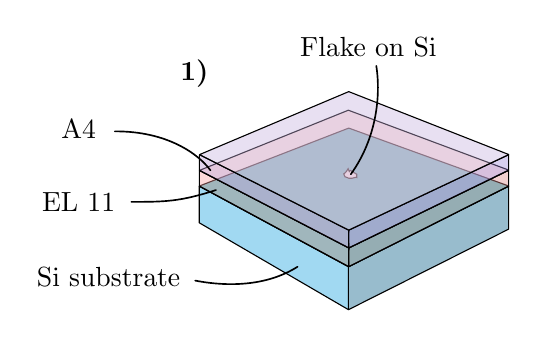
\begin{tikzpicture}

  \draw[line join=bevel, fill=cyan!89!violet!40] (-0.248,1.4) -- (-0.248,0.934) -- (1.648,-0.17) -- (1.648,0.375) -- cycle;
  \draw[line join=bevel, fill=cyan!87!purple!34!lightgray] (1.645,0.376) -- (3.68,1.4) -- (3.68,0.853) -- (1.645,-0.17) -- cycle;
  \draw[fill=teal!90!blue!68!cyan, line join=bevel, draw opacity=1, fill opacity=0.6] (-0.25,1.4) -- (1.65,2.137) -- (3.685,1.4) -- (1.65,0.377) -- cycle;  \draw[fill=white, rounded corners=0.6pt] (1.642,1.6) .. controls (1.622,1.59) and (1.592,1.55) .. (1.602,1.54) .. controls (1.602,1.52) and (1.652,1.5) .. (1.672,1.5) .. controls (1.702,1.5) and (1.752,1.52) .. (1.752,1.53) .. controls (1.752,1.55) and (1.702,1.58) .. (1.692,1.59) .. controls (1.672,1.6) and (1.652,1.59) .. cycle;
  \draw[line join=bevel, fill=pink!97!teal!84!red, fill opacity=0.4] (-0.247,1.6) -- (-0.247,1.401) -- (1.65,0.377) -- (1.648,0.615) -- cycle;
  \draw[line join=bevel, fill=red!78!cyan!60, fill opacity=0.4] (1.653,0.615) -- (3.68,1.6) -- (3.68,1.4) -- (1.65,0.376) -- cycle;
  \draw[fill=pink!97!yellow!98, line join=bevel, draw opacity=1, fill opacity=0.4] (-0.245,1.6) -- (1.645,2.364) -- (3.68,1.604) -- (1.653,0.615) -- cycle;
  \draw[line join=bevel, fill=white!87!magenta!72!blue, fill opacity=0.4] (-0.247,1.8) -- (-0.247,1.6) -- (1.65,0.615) -- (1.653,0.84) -- cycle;
  \draw[line join=bevel, fill=white!74!orange!61!blue, fill opacity=0.4] (1.648,0.84) -- (3.68,1.8) -- (3.68,1.6) -- (1.65,0.615) -- cycle;

  \draw[fill=white!94!magenta!78!blue, line join=bevel, fill opacity=0.4, draw opacity=1] (-0.245,1.8) -- (1.65,2.6) -- (3.685,1.8) -- (1.65,0.84) -- cycle;


  \node at (-1.4,0.25) {Si substrate};
  \node at (-1.78,1.2) {EL 11};
  \node at (-1.78,2.12) {A4};
  \draw[semithick, line cap=round] (-0.3,0.2) .. controls (0.1,0.123) and (0.6,0.123) .. (1,0.376);
  \draw[semithick, line cap=round] (-1.11,1.2) .. controls (-0.69,1.2) and (-0.5,1.2) .. (-0.036,1.35);
  \draw[semithick, line cap=round] (-1.32,2.095) .. controls (-0.65,2.1) and (-0.25,1.8) .. (-0.106,1.6);
  \node at (1.9,3.173) {Flake on Si};
  \draw[semithick, line cap=round] (2,2.927) .. controls (2.06,2.54) and (2,2) .. (1.676,1.55);

  \node at (-0.31,2.825) {\textbf{1)}};
\end{tikzpicture}
        \hspace*{36pt}
        \begin{tikzpicture}

  \draw[line join=bevel, fill=cyan!89!violet!40] (-0.248,1.4) -- (-0.248,0.934) -- (1.648,-0.17) -- (1.648,0.375) -- cycle;
  \draw[line join=bevel, fill=cyan!87!purple!34!lightgray] (1.645,0.376) -- (3.68,1.4) -- (3.68,0.853) -- (1.645,-0.17) -- cycle;
  \draw[fill=teal!90!blue!68!cyan, line join=bevel, draw opacity=1, fill opacity=0.6] (-0.25,1.4) -- (1.65,2.137) -- (3.685,1.4) -- (1.65,0.377) -- cycle;  \draw[fill=white, rounded corners=0.6pt] (1.725,1.993) .. controls (1.705,1.983) and (1.675,1.943) .. (1.685,1.933) .. controls (1.685,1.913) and (1.735,1.893) .. (1.755,1.893) .. controls (1.785,1.893) and (1.835,1.913) .. (1.835,1.923) .. controls (1.835,1.943) and (1.785,1.973) .. (1.775,1.983) .. controls (1.755,1.993) and (1.735,1.983) .. cycle;
  \draw[fill=pink!97!yellow!98, line join=bevel, draw opacity=1, fill opacity=0.4] (-0.25,1.6) -- (1.65,2.35) -- (3.68,1.58) -- (1.65,0.61) -- cycle;
  \draw[line join=bevel, fill=pink!97!teal!84!red, fill opacity=0.4] (-0.247,1.6) -- (-0.246,1.401) -- (1.652,0.377) -- (1.65,0.615) -- cycle;
  \draw[line join=bevel, fill=red!78!cyan!60, fill opacity=0.4] (1.653,0.615) -- (3.68,1.58) -- (3.68,1.4) -- (1.65,0.376) -- cycle;
  \draw[line join=bevel, fill=white!87!magenta!72!blue, fill opacity=0.4] (-0.247,1.8) -- (-0.25,1.6) -- (1.65,0.615) -- (1.653,0.84) -- cycle;
  \draw[line join=bevel, fill=white!74!orange!61!blue, fill opacity=0.4] (1.648,0.84) -- (3.68,1.8) -- (3.68,1.58) -- (1.65,0.615) -- cycle;
    \draw[fill=white!94!magenta!78!blue, line join=bevel, fill opacity=0.4, draw opacity=1] (-0.253,1.8) -- (1.642,2.55) -- (3.682,1.8) -- (1.647,0.84) -- cycle;


  \draw[cyan] (1.567,1.993) -- (1.9,1.893);
  \draw[cyan] (1.614,1.845) -- (1.89,2.055);
  \draw[fill=magenta!82!white!42!cyan] (0.795,1.665) -- (1.335,1.993) -- (1.614,2.013) -- (1.586,1.973) -- (1.363,1.963) -- (0.835,1.643) -- cycle;
  \draw[fill=magenta!82!white!42!cyan] (1.635,1.893) -- (1.66,1.865) -- (1.435,1.443) -- (1.382,1.48) -- cycle;
  \draw[fill=magenta!82!white!42!cyan] (1.89,1.92) -- (1.86,1.893) -- (2.235,1.543) -- (2.29,1.573) -- cycle;
  \draw[fill=magenta!82!white!42!cyan] (1.835,2.043) -- (1.86,2.013) -- (2.035,2.093) -- (2.735,1.693) -- (2.793,1.713) -- (2.035,2.138) -- cycle;
\draw[fill=black, rounded corners=0.6pt, xscale=3, yscale=3, shade, shading=axis] (1.133,1) .. controls (1.113,0.99) and (1.083,0.95) .. (1.093,0.94) .. controls (1.093,0.92) and (1.143,0.9) .. (1.163,0.9) .. controls (1.193,0.9) and (1.243,0.92) .. (1.243,0.93) .. controls (1.243,0.95) and (1.193,0.98) .. (1.183,0.99) .. controls (1.163,1) and (1.143,0.99) .. cycle;

  \draw[arrows=-Kite, solid, semithick] (1.2,2.865) -- (1.2,1.893);
  \draw[rotate=180, fill=white!94!blue!66!cyan] (-3.82,-2.547) -- (-3.93,-2.647) -- (-3.57,-2.847) -- (-3.93,-2.917) -- (-3.83,-3.047) -- (-3.52,-2.907) -- (-3.27,-3.147) .. controls (-3.24,-3.117) and (-3.22,-3.127) .. (-3.19,-3.067) -- (-3.46,-2.867) -- (-3.037,-2.7) -- (-3.1,-2.62) -- (-3.51,-2.827) -- cycle;
  \draw (3.501,2.88) ellipse [x radius=0.7cm, y radius=0.52cm];
  \draw (1.737,1.96) ellipse [x radius=0.12cm, y radius=0.13cm];
  \draw (1.683,2.075) -- (2.9,3.147);
  \draw (1.79,1.845) -- (3.555,2.36);
  \draw[fill=magenta!82!white!42!cyan] (3.4,3.147) -- (3.15,3) -- (2.9,3.147) -- (2.947,3.2) -- (3.054,3.284) -- (3.155,3.333) -- cycle;
  \draw[fill=magenta!82!white!42!cyan] (2.822,2.754) -- (3.058,2.757) -- (3.168,2.6) -- (3,2.519) -- (2.944,2.565) -- (2.868,2.664) -- cycle;
  \draw[fill=magenta!82!white!42!cyan] (4,3.24) -- (3.8,3.1) -- (3.9,2.877) -- (4.178,3) -- (4.133,3.1) -- (4.05,3.2) -- cycle;
  \draw[fill=magenta!82!white!42!cyan] (3.9,2.7) -- (3.77,2.547) -- (3.84,2.43) -- (3.93,2.47) -- (4.033,2.547) -- (4.085,2.6) -- cycle;
  \draw[fill=magenta!82!white!42!cyan] (0.786,1.737) -- (0.478,1.612) -- (0.774,1.462) -- (1.065,1.612) -- cycle;
  \draw[fill=magenta!82!white!42!cyan] (1.325,1.543) -- (1.065,1.416) -- (1.363,1.266) -- (1.62,1.393) -- cycle;
  \draw[fill=magenta!82!white!42!cyan] (2.335,1.625) -- (2.035,1.493) -- (2.335,1.333) -- (2.665,1.493) -- cycle;
  \draw[fill=magenta!82!white!42!cyan] (2.858,1.836) -- (2.575,1.693) -- (2.885,1.543) -- (3.195,1.693) -- cycle;
  \node at (3.273,3.8) {10\si{\micro\meter}$\ast$};
  \node at (4.813,0.536) {120\si{\micro\meter}$\ast$};
  \draw[line cap=round, semithick] (3.77,2.946) .. controls (3.8,3.2) and (3.73,3.4) .. (3.4,3.6);
  \draw[semithick, line cap=round] (4.55,0.853) .. controls (4.312,1.25) and (3.928,1.58) .. (2.9,1.693);
  \node (node1) at (0.95,4.38) {Electron column};

    \draw[semithick] (0.552,3.9) .. controls (0.79,3.668) and (0.934,3.387) .. (0.984,3.058) .. controls (1.14,2.993) and (1.295,2.99) .. (1.452,3.046) .. controls (1.505,3.364) and (1.632,3.65) .. (1.835,3.9);
  \draw[semithick, line cap=round] (node1.south) .. controls (1.1,4) and (1.162,3.936) .. (1.2,3.664);



  \node at (0.95,2.6) {$e^-$};
\end{tikzpicture}

         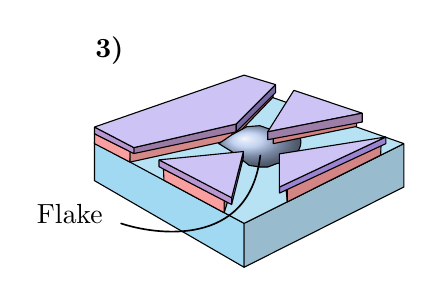
\begin{tikzpicture}

\draw[line join=bevel, fill=cyan!89!violet!40] (0,1.17) -- (0,0.68) -- (1.9,-0.42) -- (1.9,0.138) -- cycle;
\draw[line join=bevel, fill=cyan!87!purple!34!lightgray] (1.9,0.138) -- (3.93,1.15) -- (3.93,0.6) -- (1.9,-0.42) -- cycle;
\draw[fill=cyan!91!purple!31, line join=bevel, draw opacity=1, fill opacity=1] (0,1.158) -- (1.9,1.863) -- (3.93,1.15) -- (1.9,0.138) -- cycle;
\draw[line join=bevel, fill=lightgray!90!black!70!red, fill opacity=1] (1.846,1) -- (1.856,0.94) -- (1.646,0.27) -- (1.646,0.43) -- cycle;
\draw[line join=bevel, fill=pink!97!teal!84!red, fill opacity=1] (0,1.276) -- (0,1.15) -- (0.451,0.916) -- (0.453,1.05) -- cycle;
\draw[line join=bevel, fill=lightgray!95!pink!71!red, fill opacity=1] (0.453,1.05) -- (0.453,0.916) -- (1.748,1.2) -- (1.748,1.325) -- cycle;
\draw[line join=bevel, fill=gray!86!white!77!red, fill opacity=1] (2.27,1.8) -- (2.267,1.74) -- (1.748,1.2) -- (1.748,1.325) -- cycle;
\draw[fill, shade, shading=ball, ball color=blue!74!green!32] (1.742,1.05) -- (1.579,1.15) -- (1.742,1.261) -- (1.934,1.365) -- (2.1,1.378) -- (2.362,1.286) -- (2.617,1.216) .. controls (2.628,1.156) and (2.617,1.1) .. (2.582,1.05) -- (2.633,0.874) -- (2.324,0.9) -- (2.2,0.853) -- (2.1,0.853) -- (1.965,0.874) -- cycle;
\draw[line join=bevel, fill=cyan!51!magenta!81!orange, fill opacity=1] (0.5,1.1) -- (0.5,1.024) -- (1.8,1.3) -- (1.8,1.4) -- cycle;
\draw[line join=bevel, fill=purple!80!magenta!59!cyan, fill opacity=1] (2.3,1.9) -- (2.3,1.8) -- (1.8,1.3) -- (1.8,1.4) -- cycle;
\draw[line join=bevel, fill=white!87!magenta!72!blue, fill opacity=1] (0,1.361) -- (0,1.276) -- (0.5,1.024) -- (0.5,1.1) -- cycle;
\draw[line join=bevel, fill=pink!97!teal!84!red, fill opacity=1] (0.876,0.829) -- (0.882,0.685) -- (1.646,0.273) -- (1.646,0.43) -- cycle;
\draw[line join=bevel, fill=white!87!magenta!72!blue, fill opacity=1] (0.82,0.944) -- (0.82,0.857) -- (1.742,0.376) -- (1.742,0.467) -- cycle;
\draw[line join=bevel, fill=blue!70!orange!56, fill opacity=1] (1.891,1.05) -- (1.891,0.975) -- (1.742,0.376) -- (1.742,0.477) -- cycle;
\draw[line join=bevel, fill=white!77!blue!85!pink] (0.82,0.944) -- (1.891,1.05) -- (1.742,0.463) -- cycle;
\draw[fill=white!77!blue!85!pink, line join=bevel] (0,1.361) -- (0.5,1.1) -- (1.8,1.4) -- (2.3,1.9) -- (1.9,2.02) -- cycle;
\draw[fill=lightgray!99!gray!69!red, line join=bevel] (2.448,0.644) -- (2.448,0.41) -- (3.634,1.005) -- (3.64,1.15) -- cycle;
\draw[fill=pink!97!teal!84!red, line join=bevel] (2.448,0.42) -- (2.426,0.636) -- (2.448,0.706) -- (2.448,0.6) -- cycle;
\draw[fill=white!77!blue!85!pink, line join=bevel] (2.532,1.827) -- (2.2,1.3) -- (3.4,1.537) -- cycle;
\draw[fill=red!96!teal!34!lightgray, line join=bevel] (2.27,1.245) -- (2.27,1.15) -- (3.327,1.368) -- (3.332,1.45) -- cycle;
\draw[fill=cyan!56!brown!63!magenta, line join=bevel] (2.2,1.3) -- (2.2,1.2) -- (3.4,1.424) -- (3.4,1.537) -- cycle;
\draw[fill=blue!68!orange!58, line join=bevel] (3.7,1.235) -- (3.7,1.15) -- (2.35,0.522) -- (2.349,0.6) -- cycle;
\draw[fill=white!77!blue!85!pink, line join=bevel] (2.349,0.599) -- (2.349,1.02) -- (3.7,1.235) -- cycle;



  \node at (-0.314,0.26) {Flake};
  \draw[semithick, line cap=round] (2.106,1) .. controls (1.965,-0.2) and (0.74,0) .. (0.337,0.137);

  \node at (0.19,2.33) {\textbf{3)}};
\end{tikzpicture}
    \end{figure}
\end{document}